\subsection{$\mathtt{turboLIB}$}
	\begin{frame}[fragile]{$\mathtt{turboLIB}$}
		The preliminary compressor design model program \href{https://github.com/antoniopucciarelli/turboLIB}{\color{blue}{$\mathtt{turboLIB}$}} can be downloaded from GitHub.
		\begin{block}{Main objects and modules}
			\begin{itemize}
				\item \verb|turboClass.turboBlade.blade|: blade object
				\item \verb|turboCoeff|: engineering coefficients module
					\begin{itemize}
						\item \verb|losses|: losses modeling 
						\item \verb|similarity|: adimensional analysis
						\item \verb|lieblein|: blade modeling
					\end{itemize}
				\item \verb|geometry.bladeGeometry.geometryData|: airfoil object
			\end{itemize}
		\end{block}
	\end{frame}

\subsubsection{Blade number}
	{\nologo
	\begin{frame}{Blade number}
		In order to define a proper number of blades for the rotor and the stator, \textbf{Howell}'s relations have been used for the estimation of the \textbf{losses}. These relations, \cite[Ch. 6]{axial2004}, are:
		\begin{itemize}
			\item $\bar{\omega}_{profile + secondary}$, this is a relation that takes into account \textbf{profile} and \textbf{3D} losses
			\item $\bar{\omega}_{endWall}$, this is previous expalined \textbf{end wall} loss
		\end{itemize}
		
		\begin{columns}
			\column{0.5\textwidth}
			\begin{figure}
				\centering
				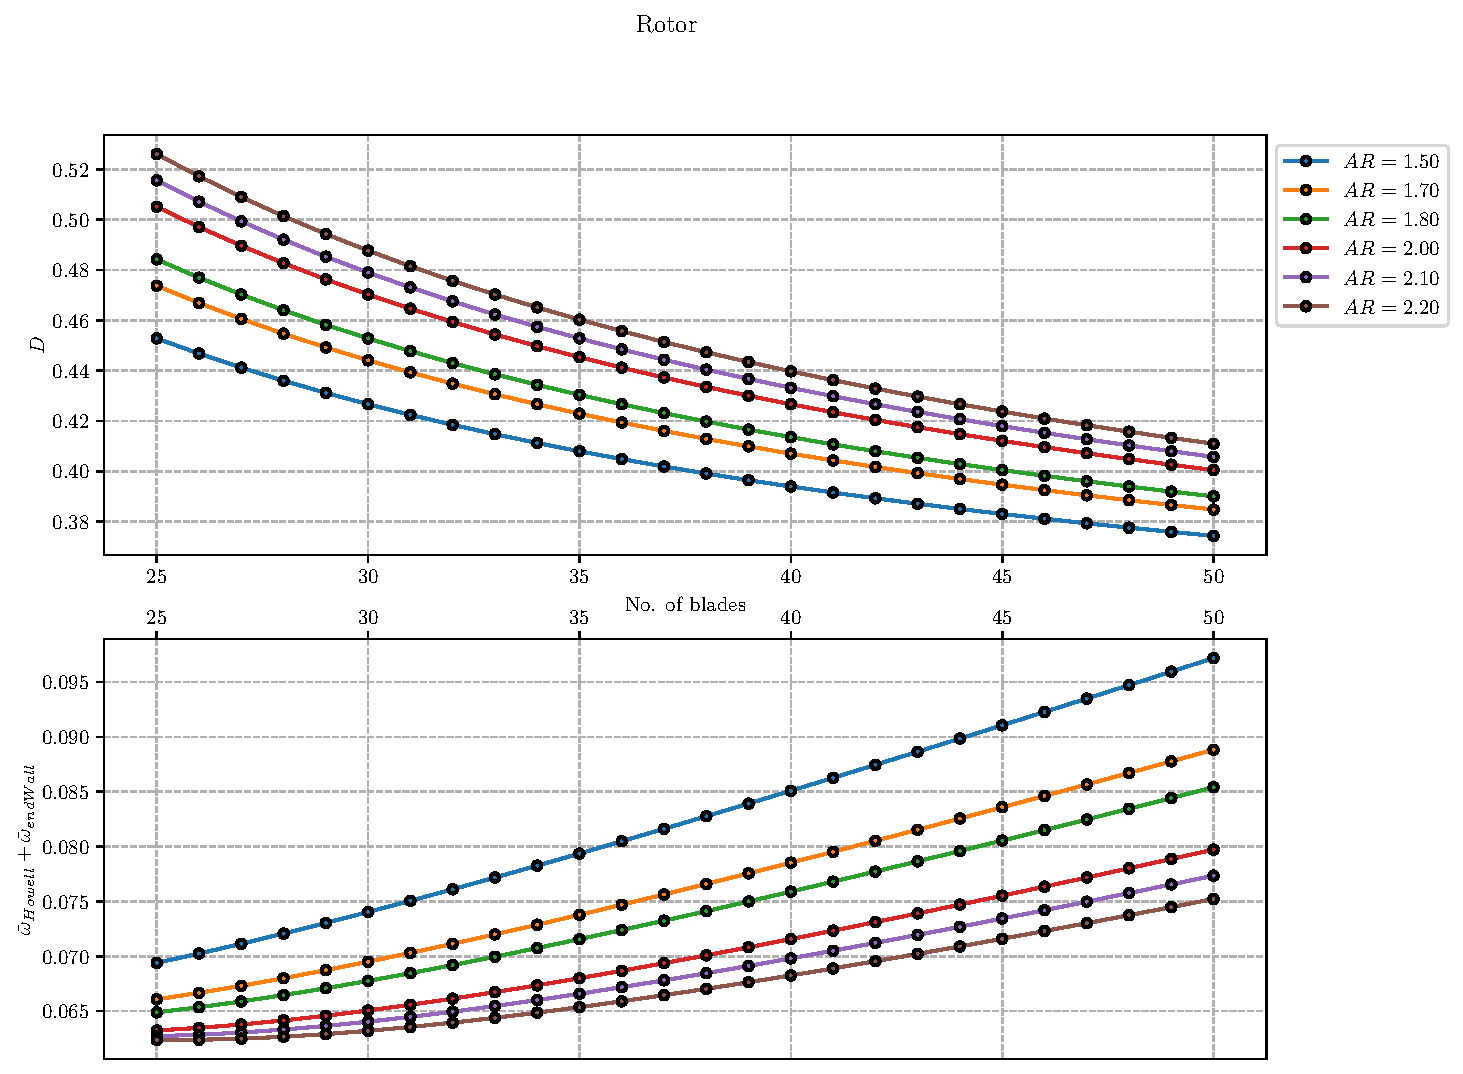
\includegraphics[width=1\textwidth]{figures/rotorBlades.pdf}
			\end{figure}
			\column{0.5\textwidth}
			\begin{figure}
				\centering
				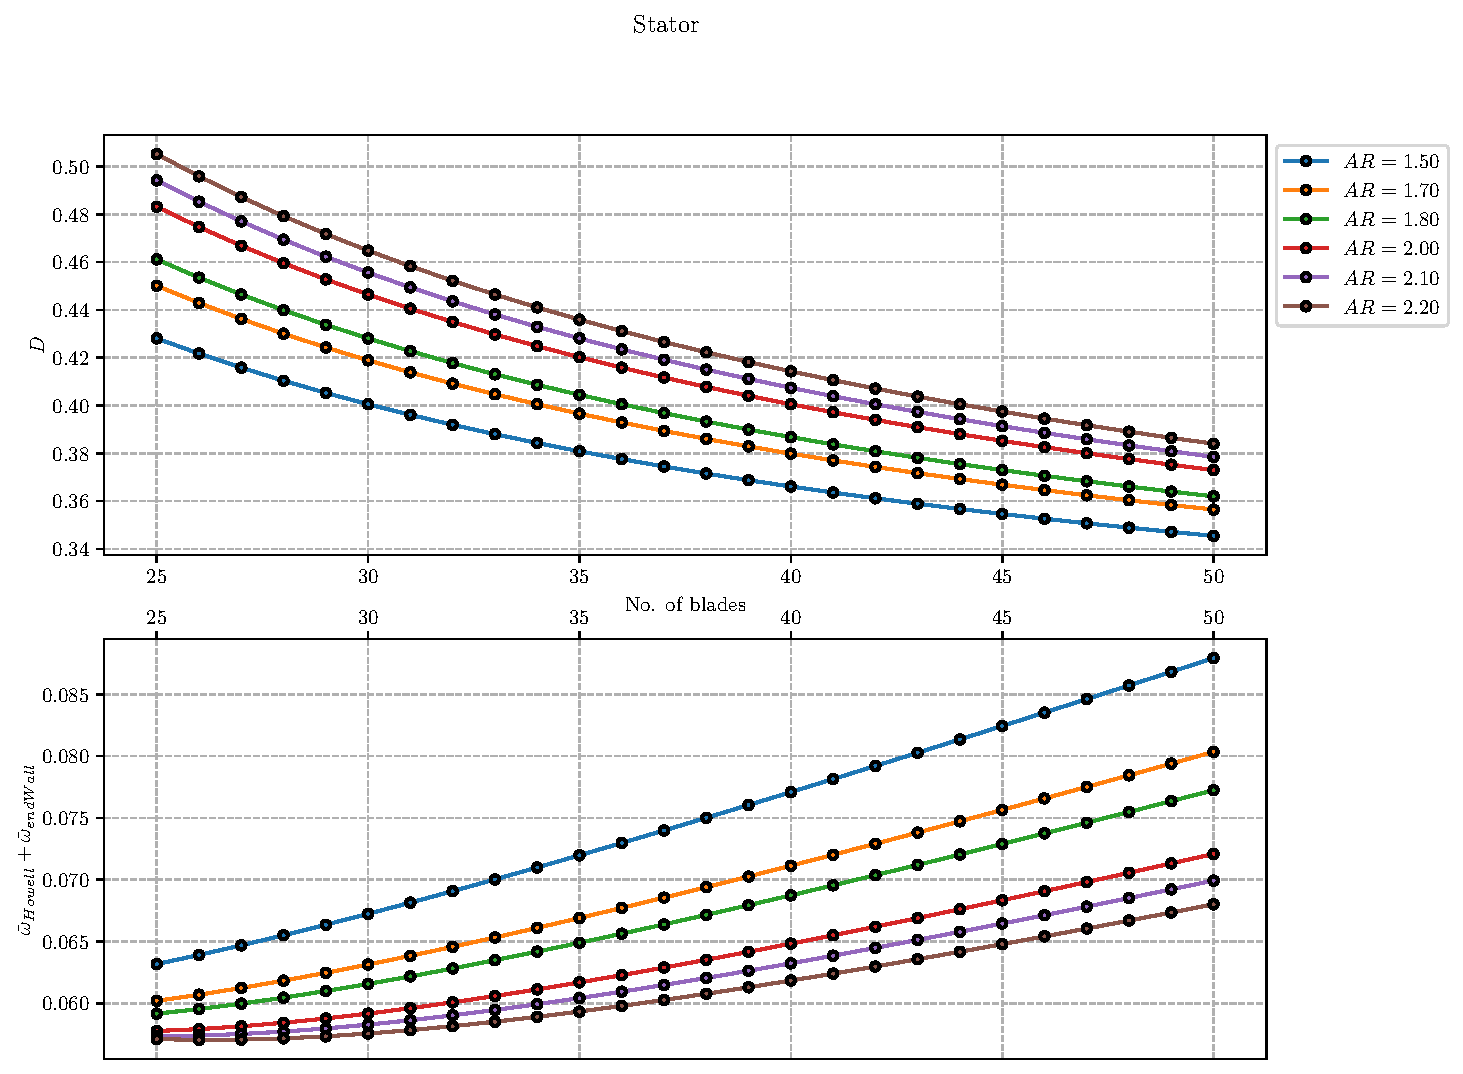
\includegraphics[width=1\textwidth]{figures/statorBlades.pdf}
			\end{figure}
		\end{columns}
	\end{frame}
	}
\subsubsection{$\mathtt{NISRE}$}
	\begin{frame}[fragile]{$\mathtt{NISRE}$}
		The \verb|NISRE| is solved through a \textbf{double nested} loop:
		\begin{itemize}
			\item \textbf{continuity loop}. Inside the \textbf{continuity loop} the \verb|scipy.integrate.odeint| function is used for the solution of the $V_{a2}^2$ \textbf{ODE}.
			\item \textbf{entropy loop}. Inside the \textbf{entropy loop} the \verb|scipy.optimize.minimize| function is used for the computation of the blade \textbf{shape}.
		\end{itemize}
	\end{frame}

\subsubsection{$\mathtt{.stl}$ \& $\mathtt{.scad}$ generation}
	\begin{frame}[fragile]{$\mathtt{.stl}$ \& $\mathtt{.scad}$ generation}
		At the end of the \verb|NISRE|, all the main blade quantities are avaliable for the \textbf{generation} of the \textbf{3D geometry}. This geometry can be converted into a \verb|.stl| file that can be used in \verb|OpenFOAM| for the flow properties study. In addition a \verb|.scad| file is made for understanding position and checking possible contacts between rotor and stator blades.	
		\newline
		\newline 
		\cite{baskharone2006principles} suggested that a good distance between rotor and stator blades is half of the rotor chord\footnote{In the radial equilibrium study losses between rotor \newline and stator blades are \textbf{neglected}.}.
	\end{frame}

\subsection{Results}
	\subsubsection{$\mathtt{NISRE}$ and main quantities}

	\begin{frame}{\textbf{Rotor} equilibrium results: $\mathtt{NISRE}$}
		\begin{figure}
			\centering
			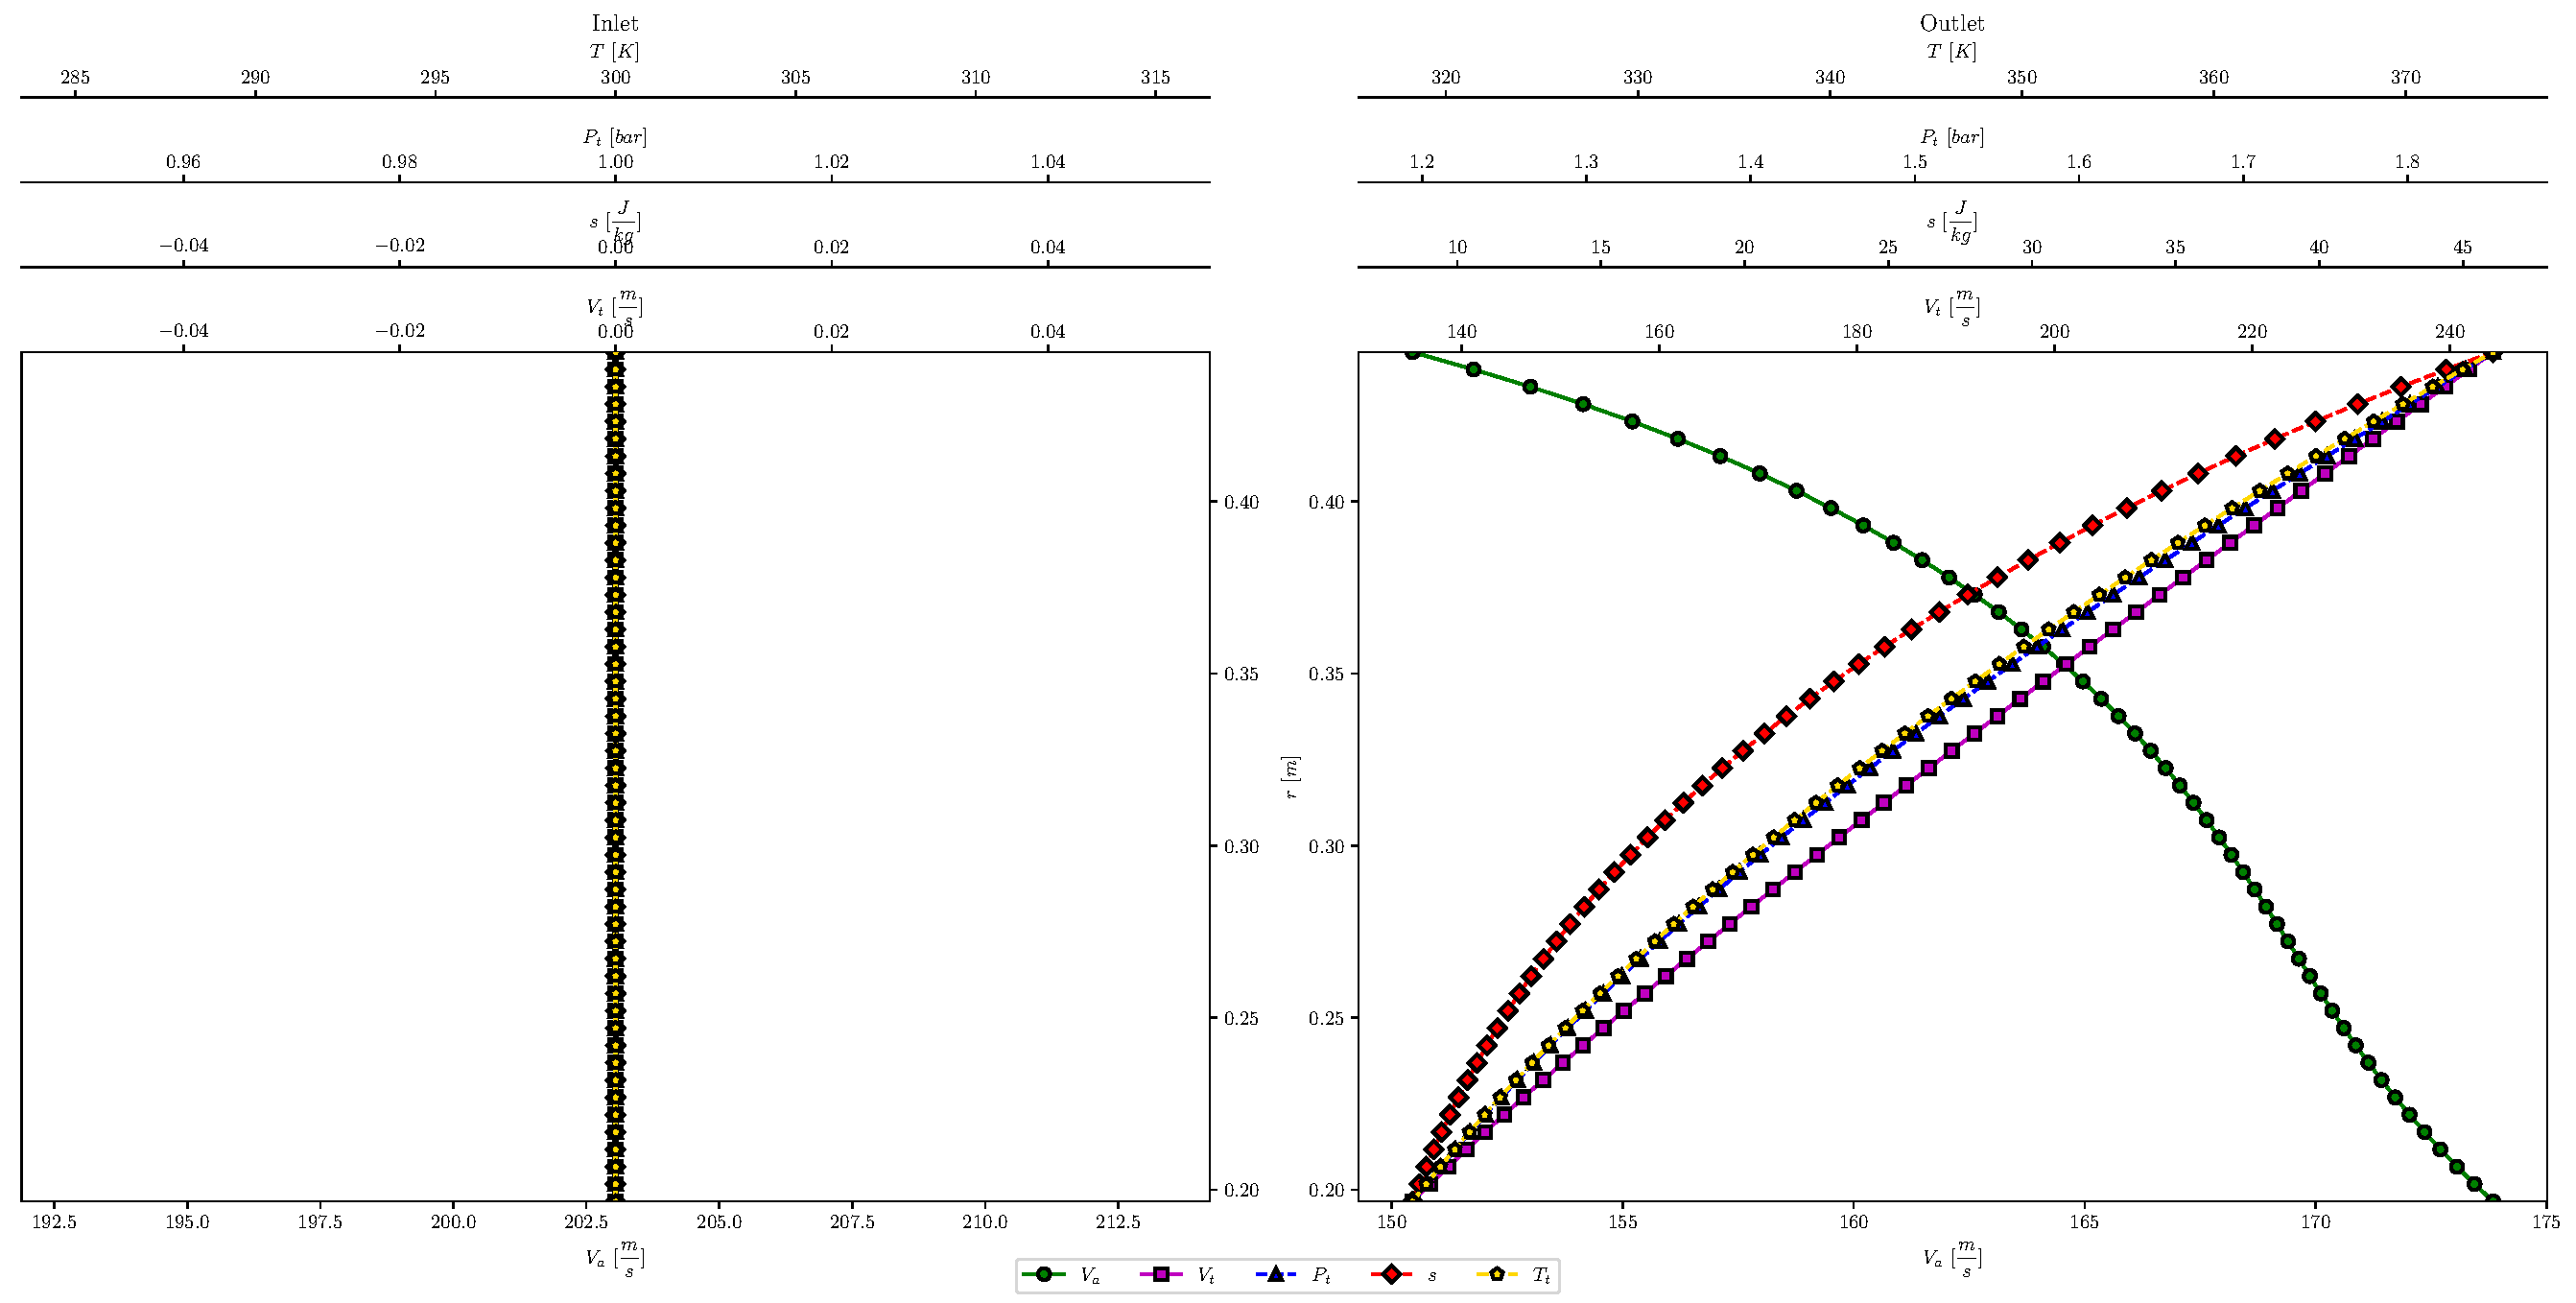
\includegraphics[width=1\textwidth]{figures/rotorEntropyFlow.pdf}
		\end{figure}
	\end{frame}
	
	\begin{frame}{\textbf{Rotor} equilibrium results: main quantities}
		\begin{figure}
			\centering
			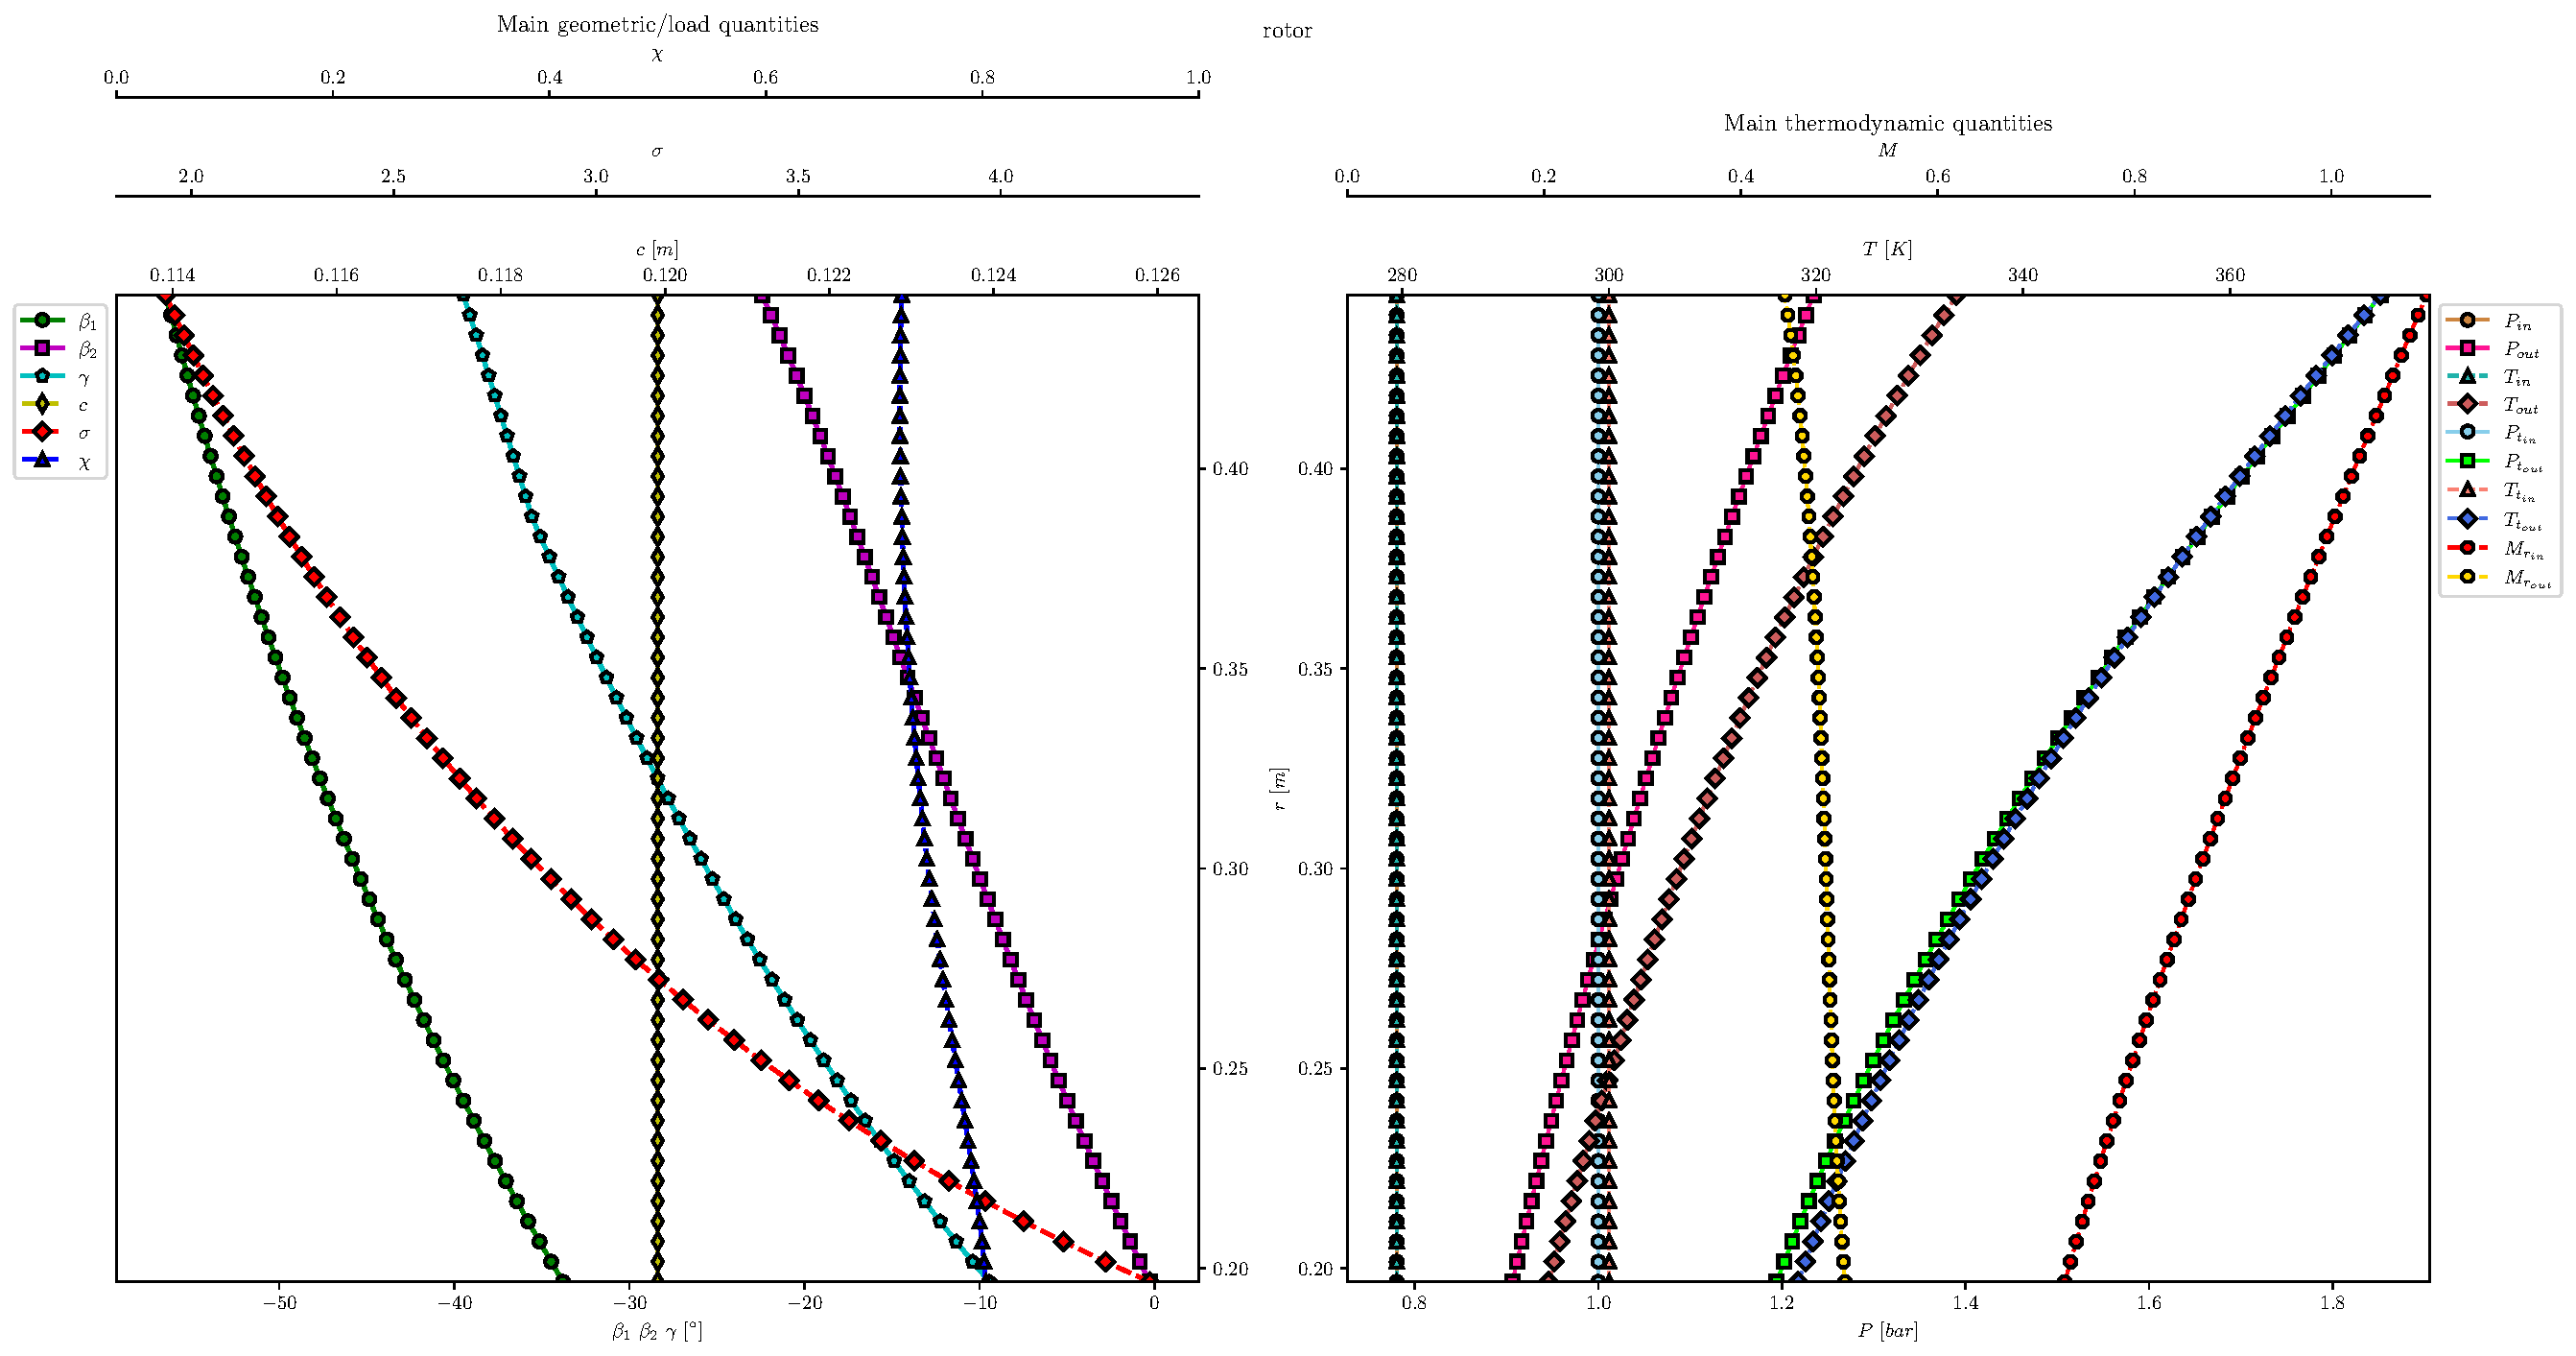
\includegraphics[width=1\textwidth]{figures/rotorBetaThermo.pdf}
		\end{figure}
	\end{frame}
	
	\begin{frame}{\textbf{Stator} equilibrium results: $\mathtt{NISRE}$}
		\begin{figure}
			\centering
			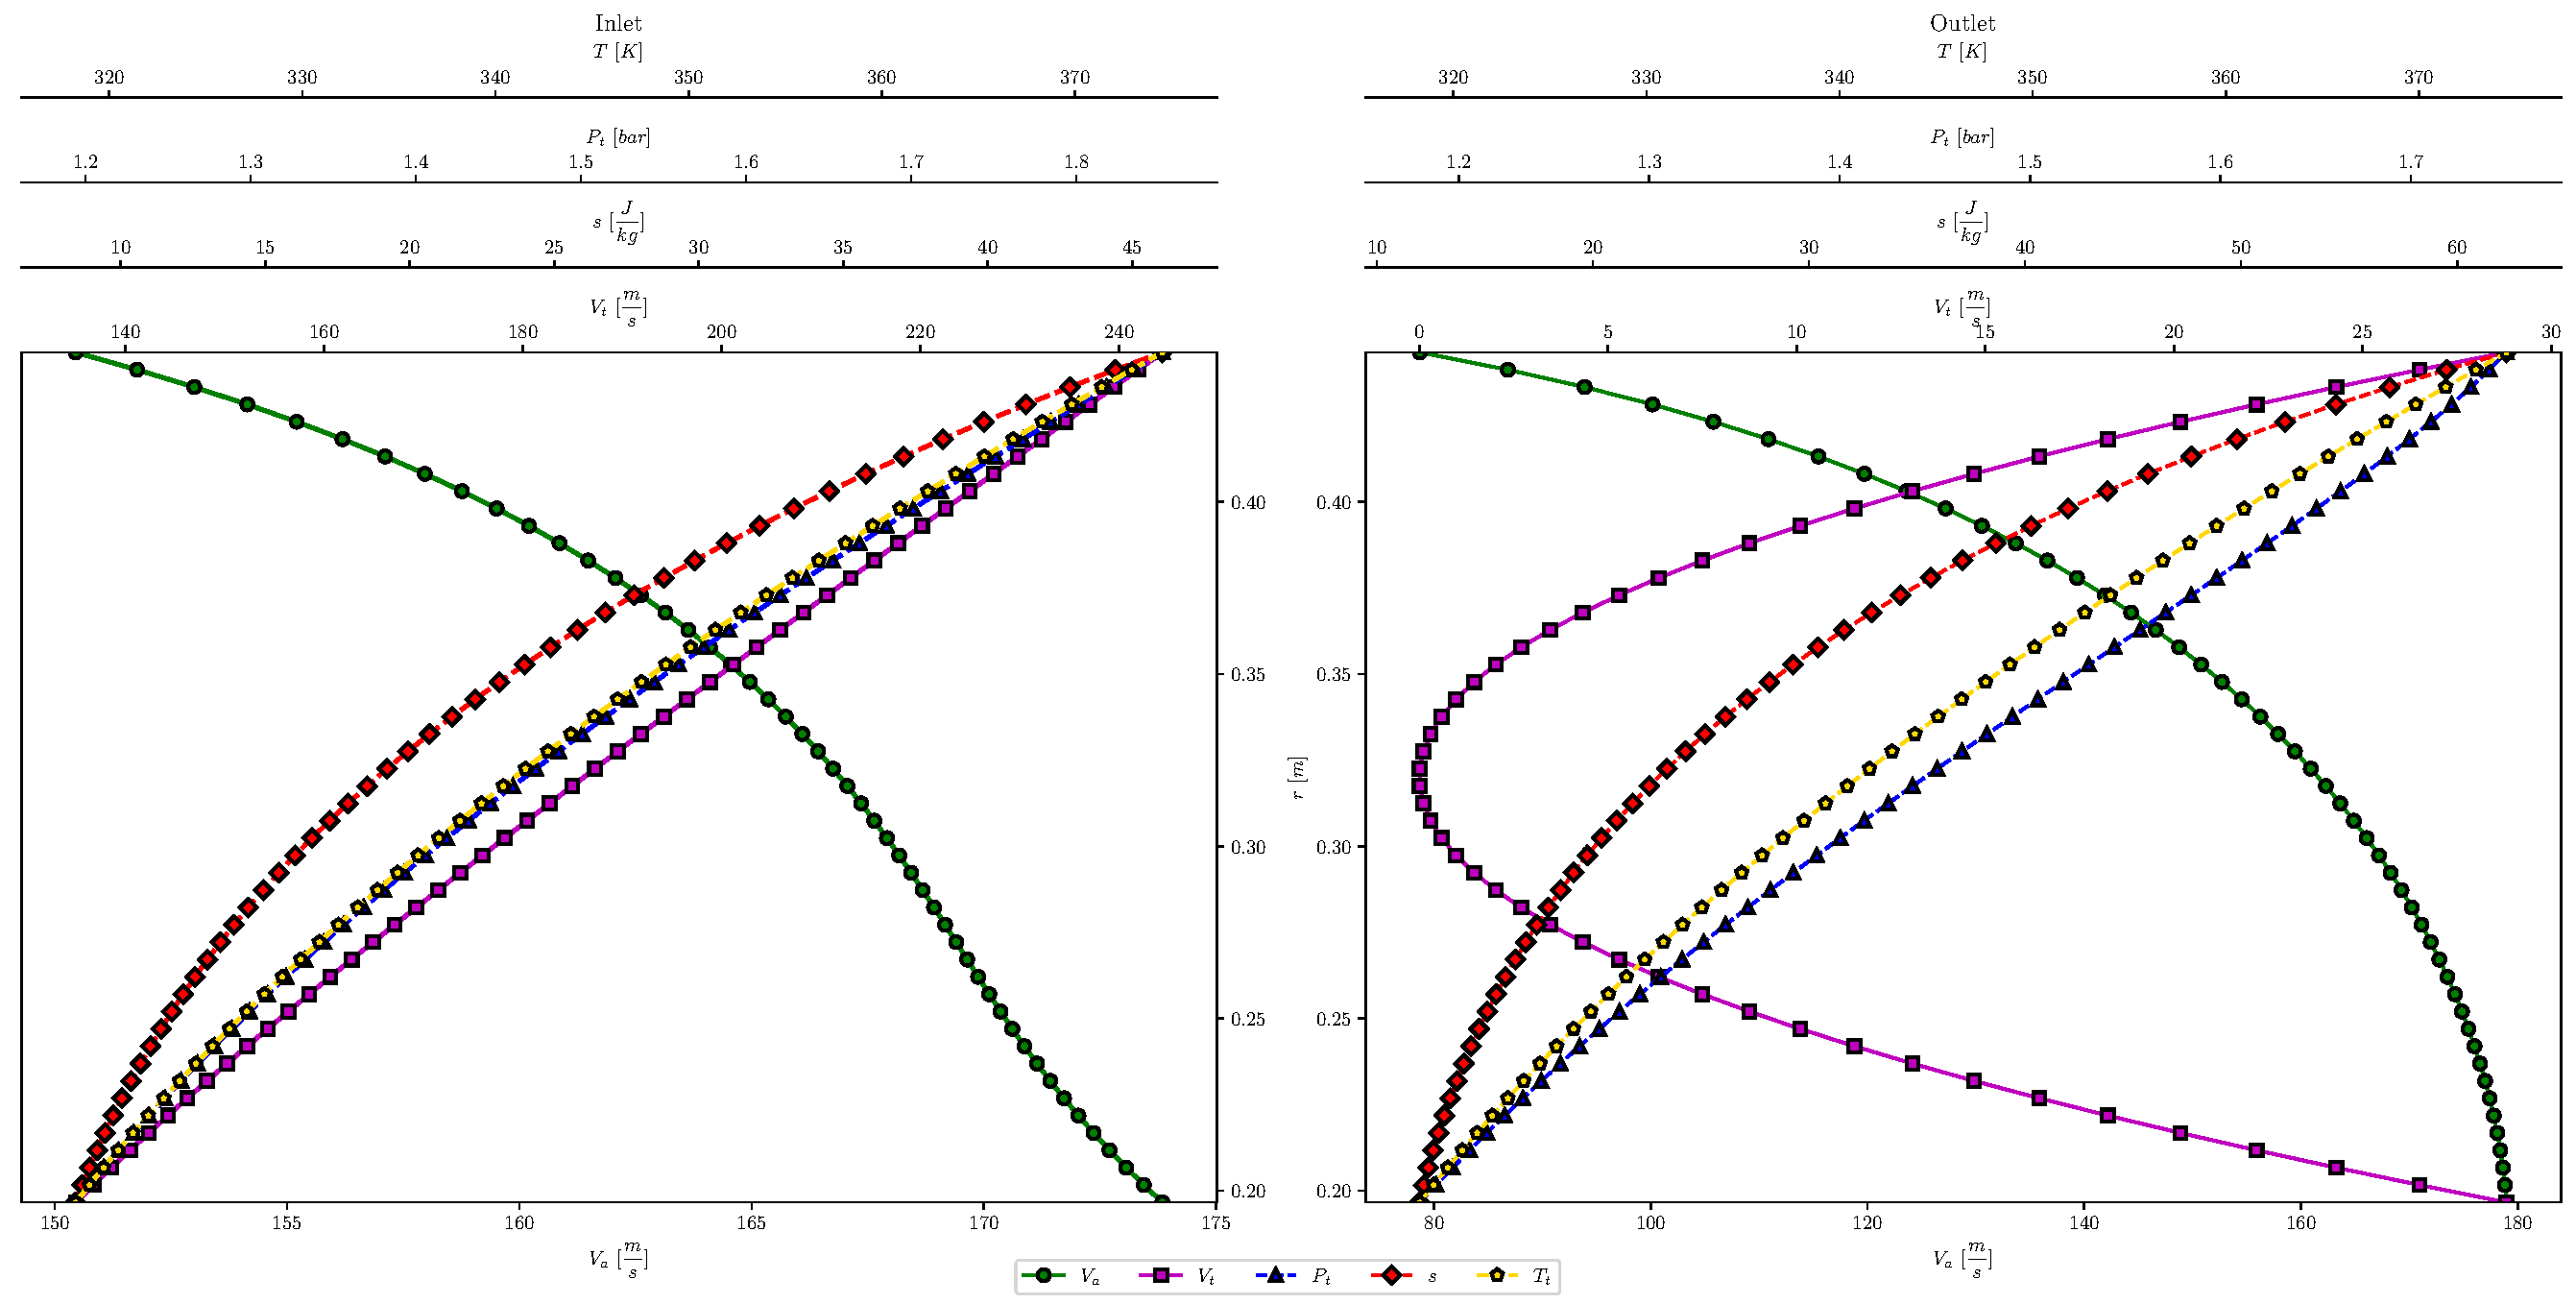
\includegraphics[width=1\textwidth]{figures/statorEntropyFlow.pdf}
		\end{figure}
	\end{frame}
	
	\begin{frame}{\textbf{Stator} equilibrium results: main quantities}
		\begin{figure}
			\centering
			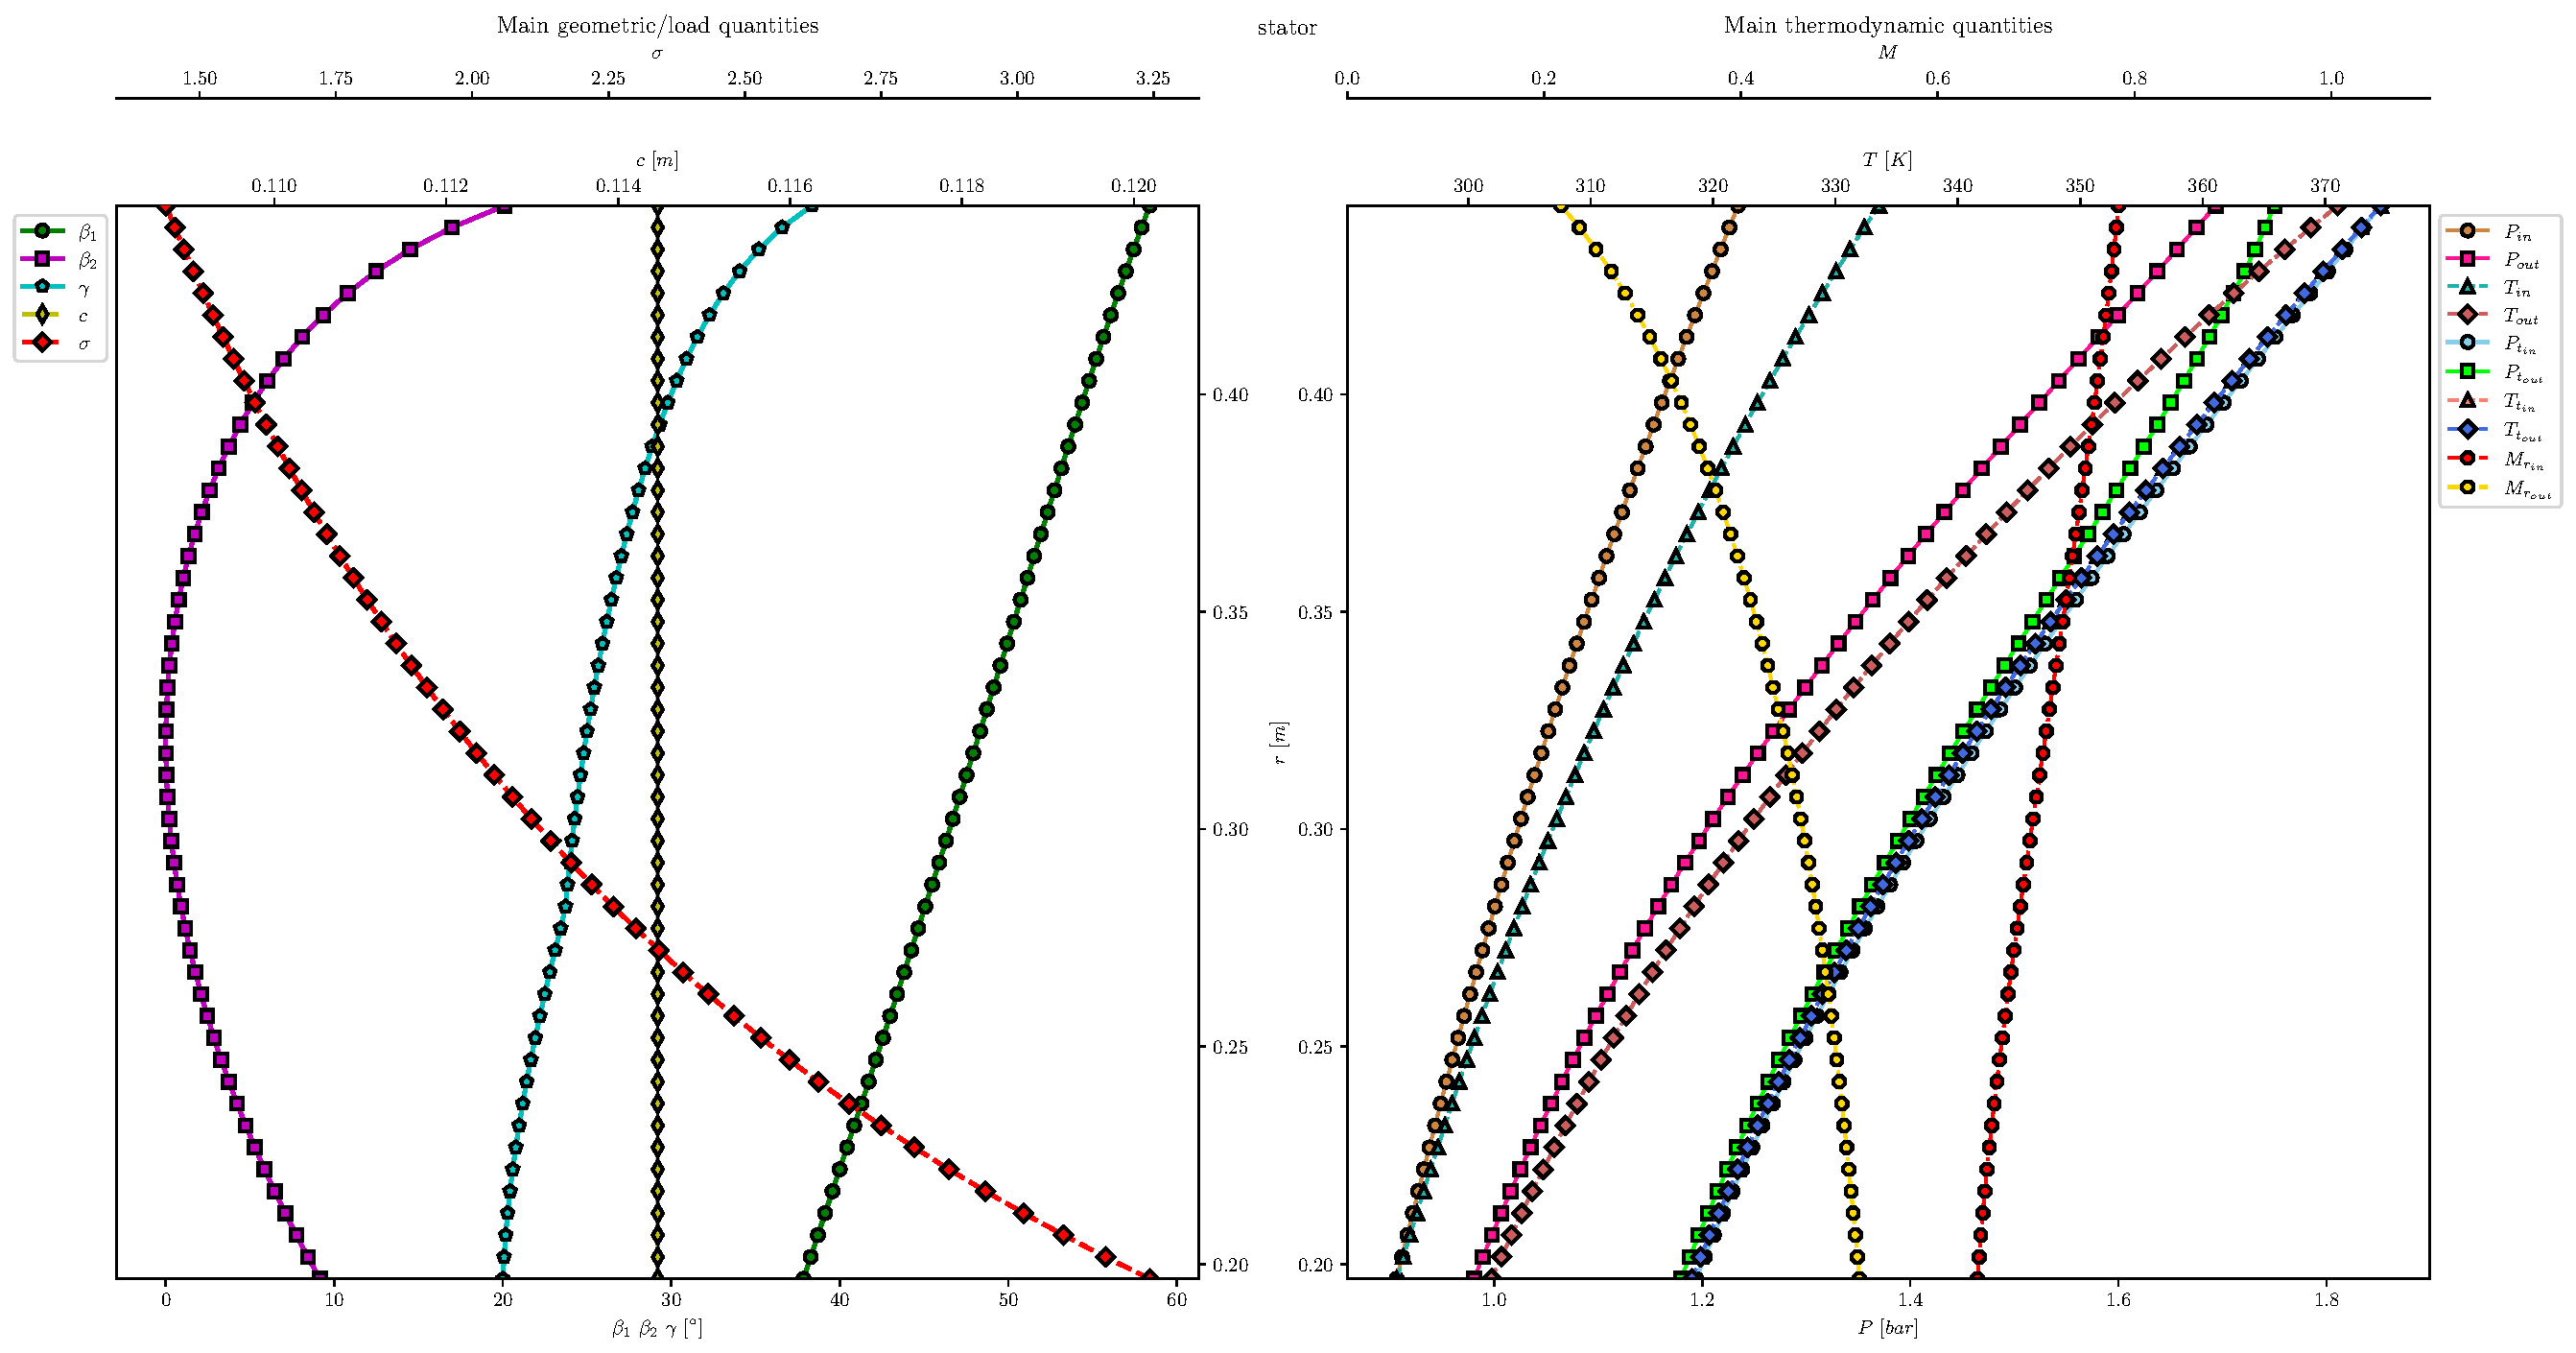
\includegraphics[width=1\textwidth]{figures/statorBetaThermo.pdf}
		\end{figure}
	\end{frame}
	
	{\nologo
	\begin{frame}{Velocity triangles}
		\begin{columns}
			\column{0.5\textwidth}
				\begin{itemize}	
					\item Inlet: \textbf{axial} velocity
					\item Outlet: \textbf{mixed vortex} model
				\end{itemize}
				\begin{figure}
					\centering
					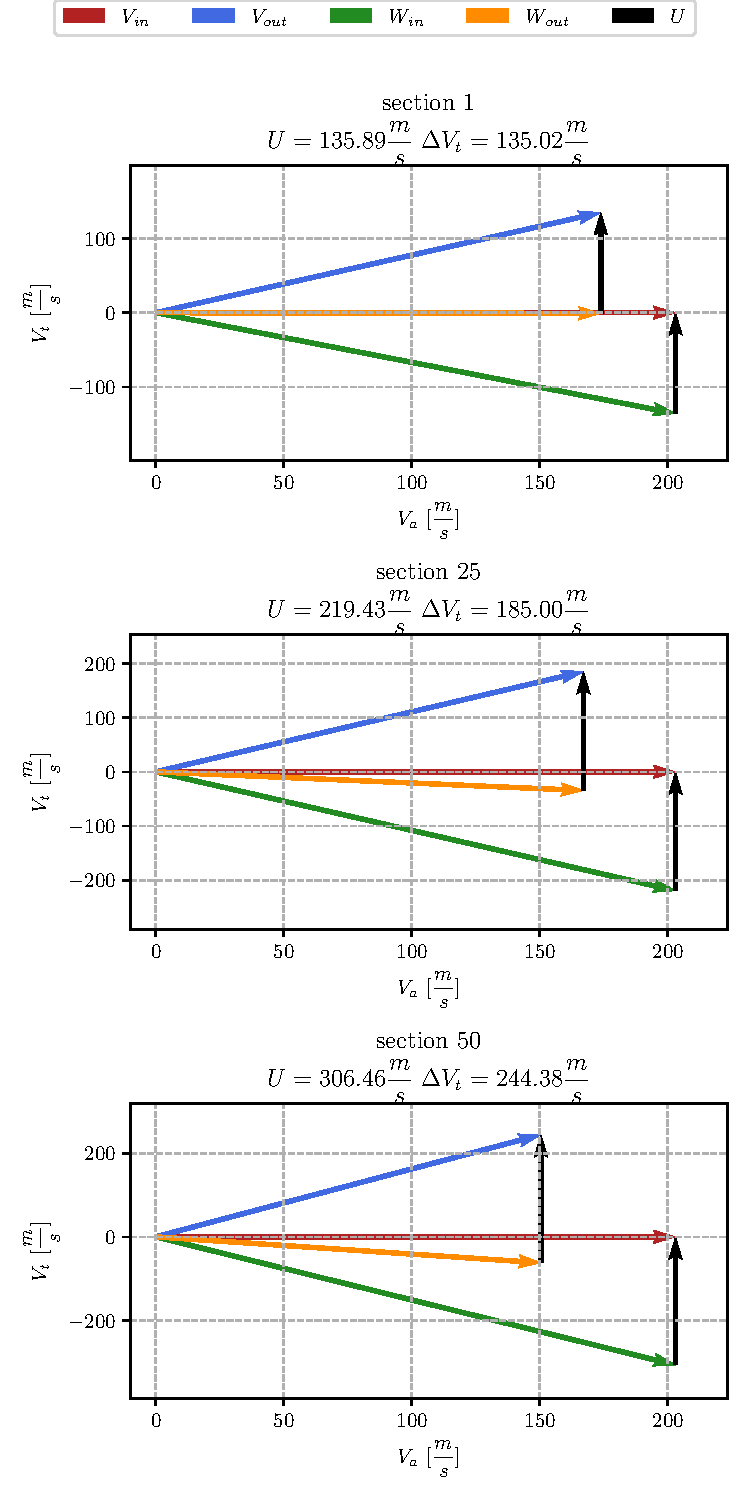
\includegraphics[width=0.5\textwidth]{figures/rotorVelocityTriangle.pdf}
				\end{figure}
			\column{0.5\textwidth}
				\begin{itemize}	
					\item Inlet: \textbf{mixed vortex} model
					\item Outlet: \textbf{second order} function 
				\end{itemize}
				\begin{figure}
					\centering
					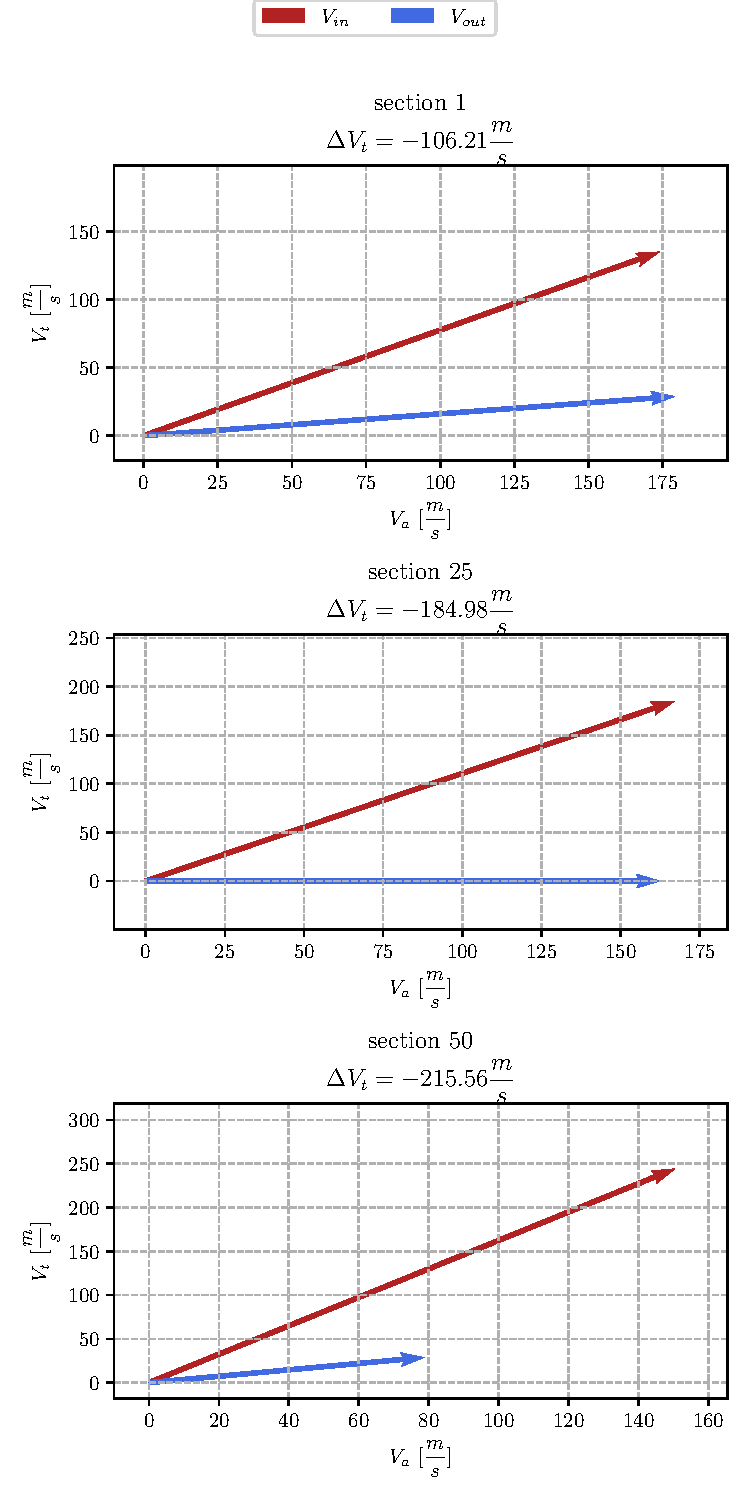
\includegraphics[width=0.5\textwidth]{figures/statorVelocityTriangle.pdf}
				\end{figure}
		\end{columns}
	\end{frame}
	}
	
	\begin{frame}{\textbf{Rotor} \& \textbf{stator} blades}
		\begin{columns}
			\column{0.5\textwidth}
				\begin{figure}
					\hspace{-2cm}
					\includegraphics[width=1.5\textwidth]{figures/rotor.png}
					\caption{Rotor blade.}
				\end{figure}
			\column{0.5\textwidth}
				\begin{figure}
					\hspace{-2cm}
					\includegraphics[width=1.5\textwidth]{figures/stator.png}
					\caption{Stator blade.}
				\end{figure}
		\end{columns}
	\end{frame}
	
	\begin{frame}{\textbf{Stage} plot}
		\begin{figure}
			\centering
			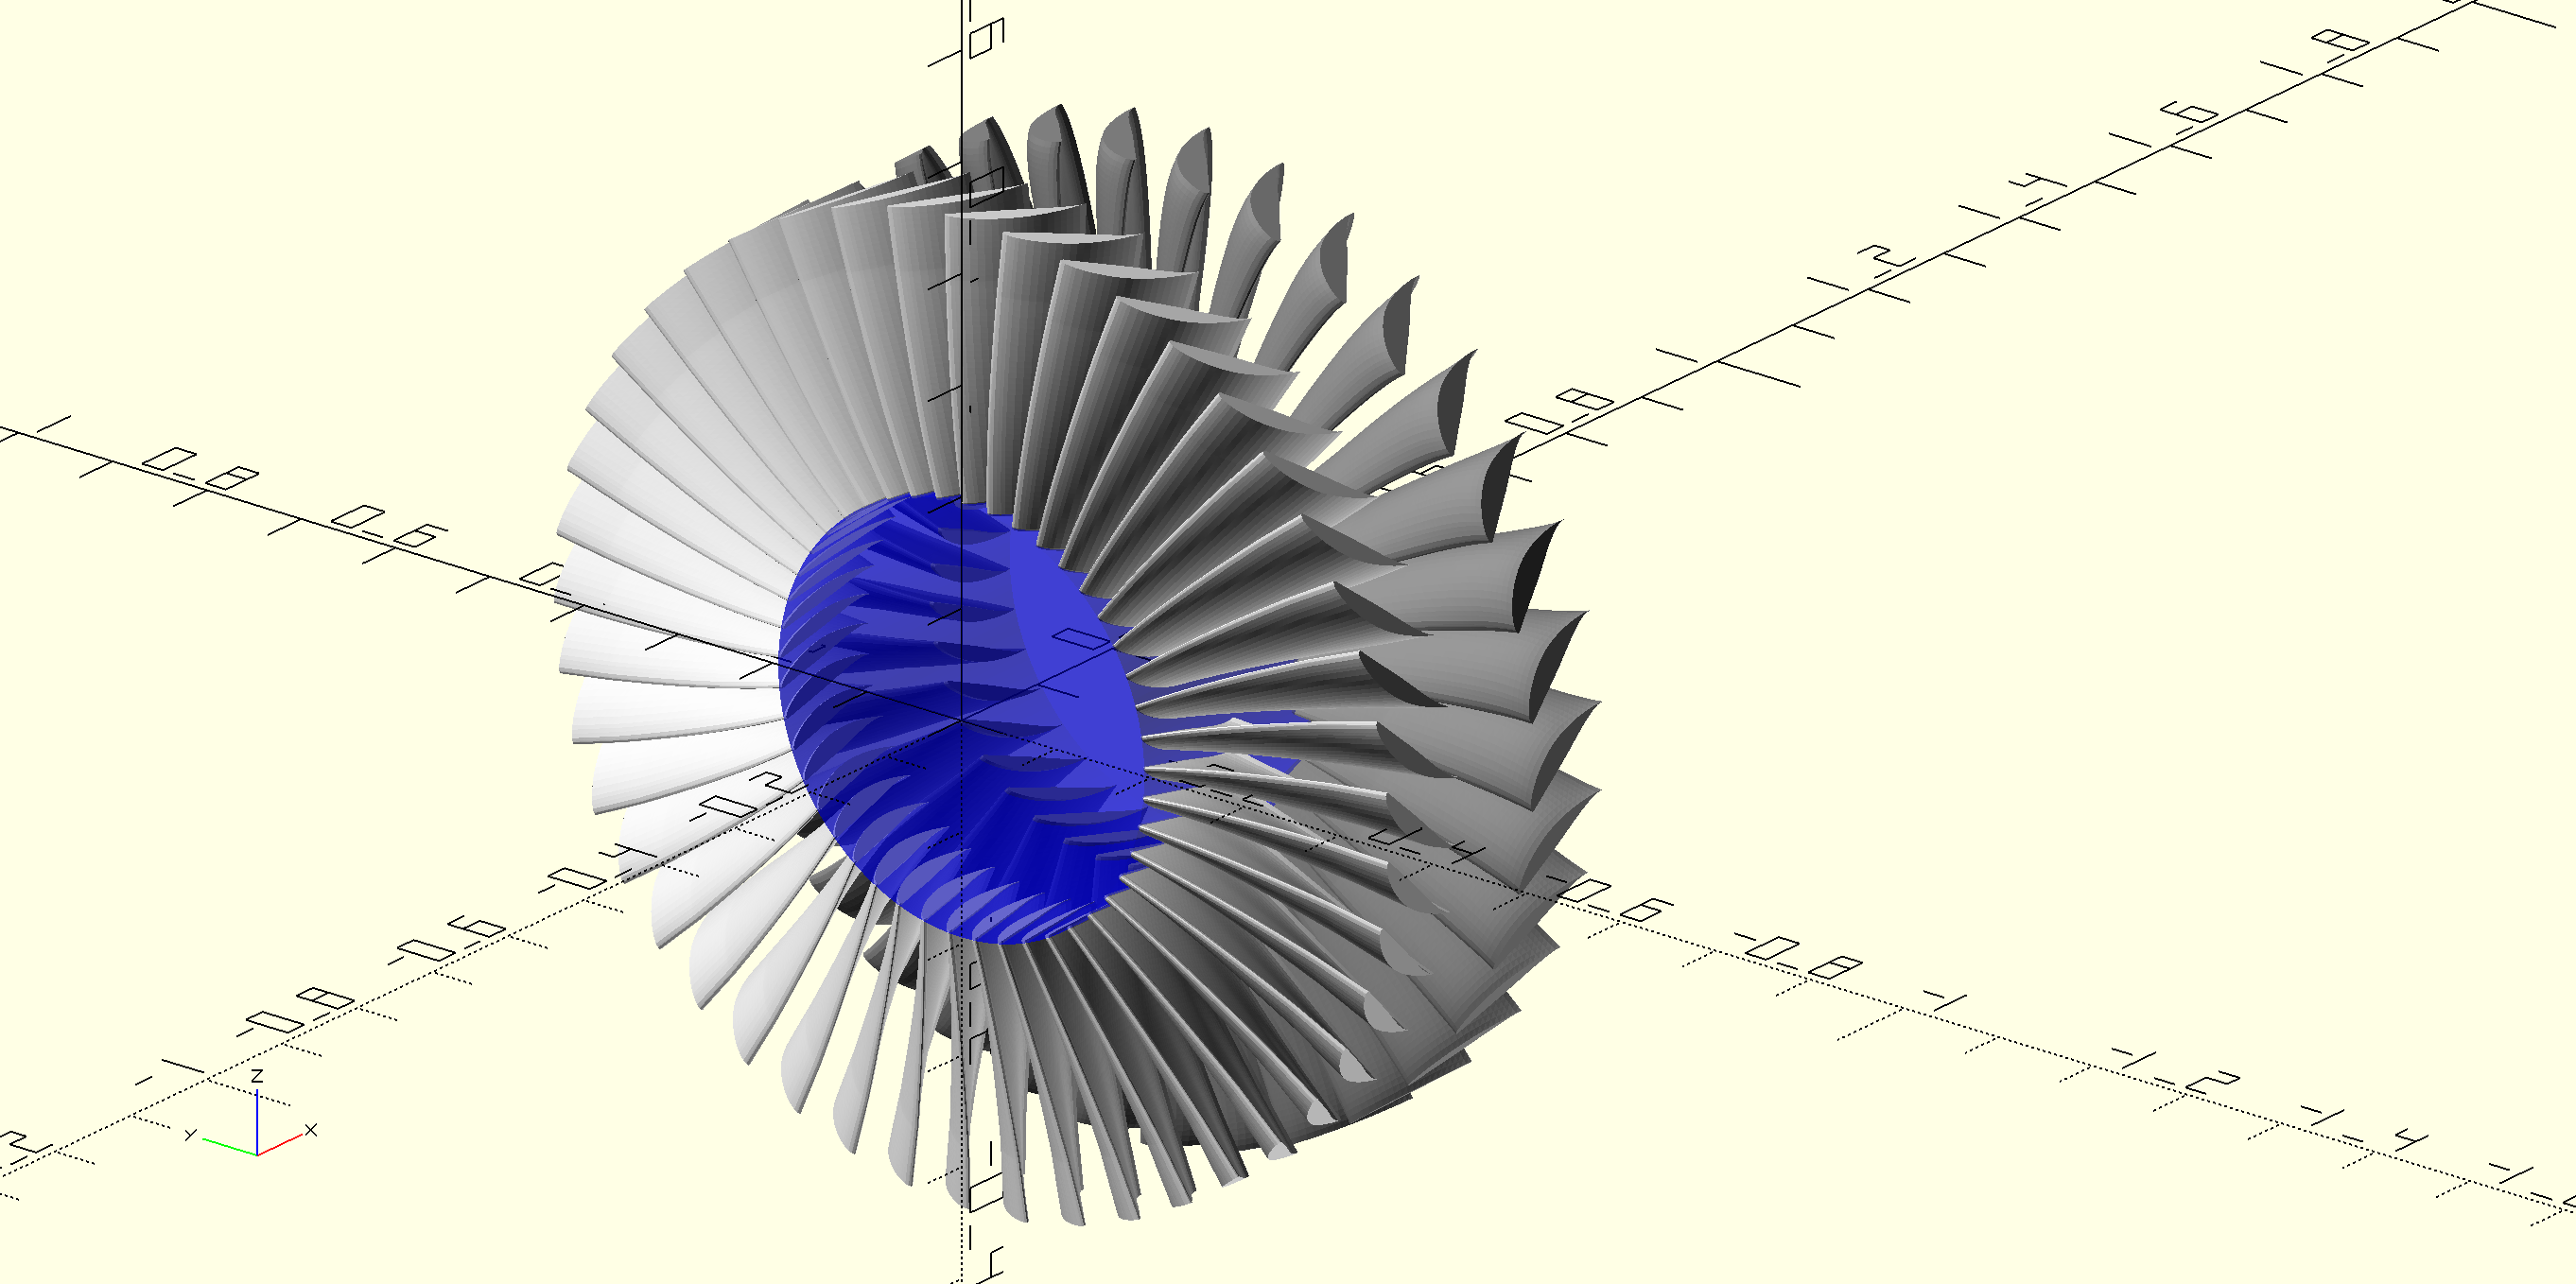
\includegraphics[width=1\textwidth]{figures/compressor.png}
		\end{figure}
	\end{frame}

\subsubsection{Efficiency}
	\begin{frame}[fragile]{Efficiency}
		The \textbf{rotor} efficiency is computed with:
		\begin{equation}
			\eta_{is_{rotor}} = \frac{W_1^2 - W_{2_{is}}^2}{W_1^2 - W_{2}^2} \nonumber 
		\end{equation}
		The \textbf{stator} efficiency is computed with:
		\begin{equation}
			\eta_{is_{stator}} = \frac{\Delta h_{is}}{\Delta h_{real}}
			\nonumber 
		\end{equation}
		The modeling results are stored into \verb|compressor_0.58_0.32_45_35.txt|.
	\end{frame}
